\section{Обходы графа II}
\subsection{Условие задания}
\textbf{Вариант 5:} Подсчитать количество связных компонент графа.

\subsection{Примеры исходного кода}
Для нахождения компонент связности графа был описан метод\\
\mitext{connectedComponents()}:
\begin{minted}{typescript}
connectedComponents(): number {
  const visited: Set<string> = new Set()

  let count = 0 // количество компонент
  for (const node of this.adj.keys()) {
    if (!visited.has(node)) { // если еще не посетили, выполнить DFS
      count++ // новая компонента
      this.dfs(node, visited) // DFS посещаем все узлы в этой компоненте связности
    }
  }

  return count
}
\end{minted}

А также вспомогательный метод обхода в глубину:
\begin{minted}{typescript}
private dfs(node: string, visited: Set<string>) {
  visited.add(node)

  const neighbors = this.adj.get(node)!
  for (const neighbor of neighbors.keys()) {
    if (!visited.has(neighbor)) {
      this.dfs(neighbor, visited) // рекурсивно обойти соседние узлы
    }
  }
}
\end{minted}

\subsection{Краткое описание алгоритма}
Вводится счетчик количества компонент связности. Также ведется множество
уже посещенных вершин. Алгоритм заканчивает работу, когда все вершины посещены.
На каждой итерации выбирается непосещенная вершина и с помощью обхода
в глубину посещаются все связные с ней вершины (одна компонента связности).
Таким образом, мы сможем подсчитать, сколько всего компонент связности
в графе.

\subsection{Примеры входных и выходных данных}
\subsubsection{Входные данные}
\begin{figure}[H]
  \begin{minipage}{0.5\textwidth}
    \centering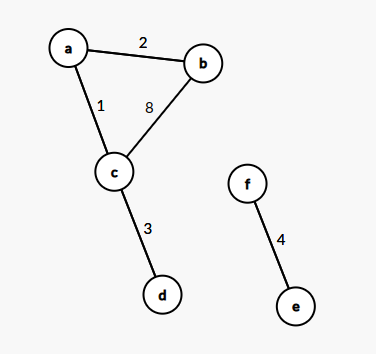
\includegraphics[width=0.6\linewidth]{figs/task-5/graph-5.png}
  \end{minipage}
  \begin{minipage}{0.5\textwidth}
    \centering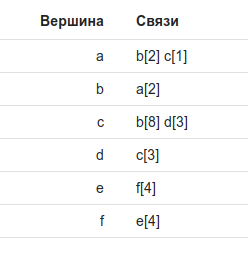
\includegraphics[width=0.6\linewidth]{figs/task-5/adj-5.png}
  \end{minipage}
  \caption{Неориентированный граф}
\end{figure}

\begin{minted}{js}
{
  "weighted": true,
  "oriented": false,
  "adj": {
    "a": {
      "b": 2,
      "c": 1
    },
    "b": {
      "a": 2
    },
    "c": {
      "a": 1,
      "d": 3
    },
    "d": {
      "c": 3
    },
    "e": {
      "f": 4
    },
    "f": {
      "e": 4
    }
  }
}
\end{minted}

\subsubsection{Выходные данные}
\begin{figure}[H]
  \centering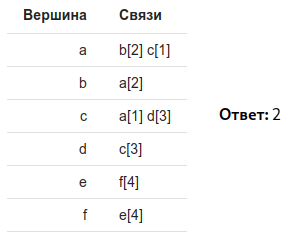
\includegraphics[width=0.4\textwidth]{figs/task-5/res-5.png}
  \caption{Результат работы}
\end{figure}